\documentclass[11pt]{article}

\usepackage{setspace}
\usepackage[margin=1in]{geometry}

% Make table of contents look better
\usepackage{tabularx}
\usepackage{tocloft}
\renewcommand{\cftsecleader}{\cftdotfill{\cftdotsep}}

\usepackage{graphicx}
\usepackage{pdfpages}
\usepackage{hyperref}

% \usepackage[ngerman]{babel}
% \usepackage[T1]{fontenc}
% \usepackage[ansinew]{inputenc}
% \usepackage{lmodern}

% Times New Roman font
\usepackage{txfonts}

\begin{document}

\setlength{\parindent}{2em}

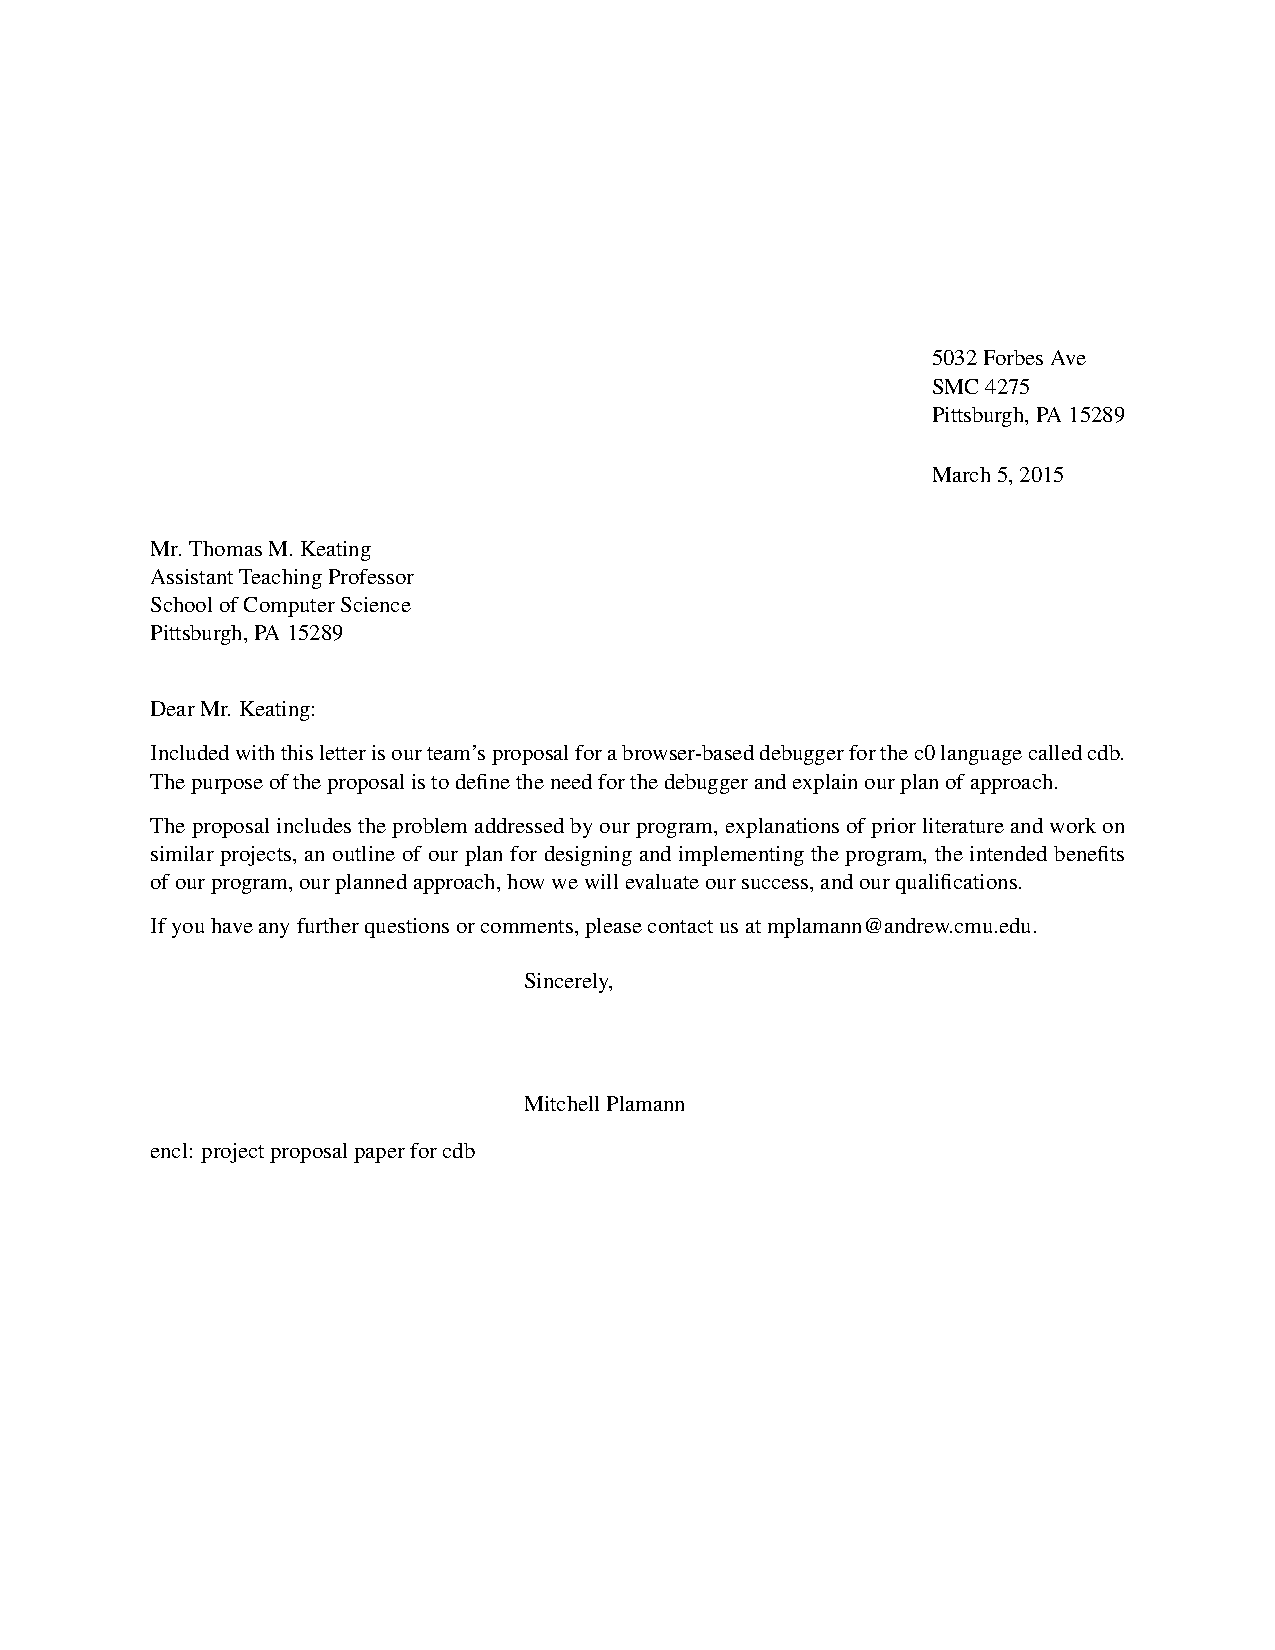
\includepdf[pages={1}]{letter.pdf}

\begin{titlepage}
\clearpage
\thispagestyle{empty}

\begin{center}
{\bf Project Proposal}\\
\vspace{10 mm}
{\bf C0 Debugger}\\
\vspace{10 mm}

Submitted to\\
Mr. Thomas M. Keating\\
Assistant Teaching Professor\\
School of Computer Science\\
Pittsbugh, PA 15289

\vspace{10 mm}

Prepared by\\
{\bf Mitchell Plamann}\\
Shyam Raghavan\\
{\bf Suhaas Reddy}\\
Aaron Gutierrez

\vspace{10 mm}

School of Computer Science\\
Carnegie Mellon University\\
March 5, 2015

\vspace{10 mm}

{\bf Abstract}
\end{center}
\par
This project is a proposal for C0 Debugger, a browser-based debugger for the
C0 programming language.
Students in Carnegie Mellon University's 15-122: Principles of Imperative
Computation and other classes learn to program in C0.
This project will allow students to better write C0 code by providing a 
powerful and easy-to-use system for debugging their C0 programs.
This proposal goes over a detailed plan for how our team will create the C0 Debugger.
\end{titlepage}

\pagenumbering{roman}
\tableofcontents
\newpage

\pagenumbering{arabic}

\section{Introduction}
One of Carnegie Mellon University's most widely attended classes is 15-122,
Principles of Imperative Computation. 15-122 contains a capstone assignment
called the C0 Virtual Machine, which involves implementing a program that
allows the user to run arbitrary code in C0, the language in which 15-122 is
taught. The implementation of the virtual machine (C0VM) is not an easy
task - it involves higher level thinking and a deep understanding of the
abstractions associated with running arbitrary code. Because it is difficult,
the CDB (C0 Debugger) hopes to improve the learning process by making
visualization and interaction with a working implementation of the C0VM more
accessible to 15-122 students. This involves creating a working Javascript
version of the C0VM, implementing visualizers for relevant parts of the
assignment, and developing the interface for student-based interaction with
the application. With development time and effort, the CDB has the opportunity
to change the future of imperative computation education.

\section{Literature Review}
\par
Here we will discuss projects similar to ours, as well as technology
we plan to use for our project.
\begin{itemize}
\item Building an In-Browser JavaScript VM and Debugger Using Generators\\
  http://amasad.me/2014/01/06/building-an-in-browser-javascript-vm-and-debugger-using-generators/
  \par
  In this blog post, Amjad Masad describes how he implemented
  debug.js, a JavaScript debugger running inside the web
  browser. Since we wish to implement a C0 debugger running inside the
  web browser, Masad's notes seem to be relevant.  Specifically, this
  post discusses the architecture of debug.js, as well as various
  challenges Masad faced in developing it.  Debug.js was designed in
  two separate parts: a virtual machine and a debugger. The virtual
  machine handled the task of evaluating the JavaScript program being
  debugged, adding support for stopping, starting, and analyzing the
  program. The debugger was the visual interface to the virtual
  machine, allowing users to control the virtual machine and see its
  output. We may wish to design our project similarly.
  \par
  Masad also discusses challenges he overcame while writing
  debug.js. These included being able to step line-by-line through a
  program, keeping track of a call stack, handling errors and
  exceptions, implementing native APIs, and dealing with events. While
  many of the details will be different when working with C0, we must
  still consider all of these challenges in developing our project.

\item The Architecture of Open Source Applications (Volume 2): Processing.js\\
  http://www.aosabook.org/en/pjs.html
  \par
  In Chapter 17 of Mike Kamermans' book {\it The Architecture of Open
  Source Applications}, he discusses the design of
  Processing.js. Processing is a Java-based programming language
  designed to help teach computer programming in a visual
  context. Processing.js is a project designed to run Processing
  programs in the web browser using only JavaScript.  This was done by
  writing a Java-to-JavaScript compiler, and running the resulting
  code attached to a HTML canvas.  Along the way, the developers ran
  into several different challenges, mostly due to differences between
  the Java and JavaScript languages.  The largest difference between
  the languages was that JavaScript programs do not get their own
  thread; the browser freezes if a JavaScript program tries to run for
  too long.  We must consider this issue among others for our project.

\item Node.js Documentation\\
  http://nodejs.org/documentation/
  \par
  This is the documentation for the node.js platform.  We plan to use
  node.js to write the server-side code for our project.  We believe
  that node is a good fit for our project since we are writing
  JavaScript for the client side of our code, so this will let us work
  in the same language on the server and client side.  Also, we can
  make use of the existing cc0 compiler to translate C0 source code to
  the bytecode our virtual machine will run. This is the same compiler
  used in 15-122, and integrating it with our server will make it
  feasible to run actual C0 source code.
\end{itemize}
\section{Plan}
\par
Our goal is to build a web application that can debug C0 code.
The user will type in or upload C0 source files.
Once this is done, these files will be transferred to our server,
where the existing cc0 compiler will be used to
generate bytecode corresponding to the user's source code.
This bytecode will be sent back to the user's web browser,
where we will be running a C0 virtual machine.
The user will be able to control this virtual machine as it executes their code. 
This will give the user the ability to run their code line-by-line,
to set breakpoints, view stack traces, and see the values of variables.
By providing access to all this information,
we hope to make it easier for users to write and debug C0 programs.
\par
For version control, we will use a git repository hosted on GitHub. 
We will use a Gantt chart, shown later in this proposal, to stay on schedule.


\section{Benefits}
\par
This project will benefit students in 15-122 Principals of Imperative
Computation at Carnegie Mellon University by helping them create correct
programs. The C0 Debugger will enable students to understand how their programs
execute and find where problems originate more easily than with existing tools.
In addition to debugging, students will have better knowledge for how the
underlying computation model works when evaluating their code.
\par
The C0 Debugger will also enable students to test simple programs with little
setup, using only a web browser. They will no longer have to set up and become
familiar with a Unix environment before they can program, making C0 accessible
to more people, more quickly.

\section{Approach}
\par
The approach section contains our methodology, how we plan to implement the
project, our project schedule, and the timeline we plan to adhere to.  The
methodology outlines the specific tools we will use to complete the project in
a timely manner whereas the schedule outlines the deadlines by which we hope to
have certain tasks completed.

\subsection{Methodology}
The C0 Debugger is designed for the CMU teaching language, C0.  It will be
hosted on Heroku with the website itself designed in CSS and HTML, using
Node.js to run most of the core functionality.  We will first deploy a blank
template website after which half of the team will work on parsing C0 bytecode
and the other half will work on creating a meaningful user experience.  Once
both teams have made reasonable progress, they will combine the two units to
complete the basic outline of the project.

\subsection{Project Schedule}
The project will be separated into five main phases: basic website design,
backend implementation, frontend implementation, user testing, and revisions.
The first phase should take less than a week with the
next two phases occurring simultaneously and composing the rest of the month's
work.  User testing and revisions will then take up the
remainder of the alloted time, with extra time padded in case implementation or
revisions are more extensive than we have predicted.
\begin{figure}[h]
  \centering
  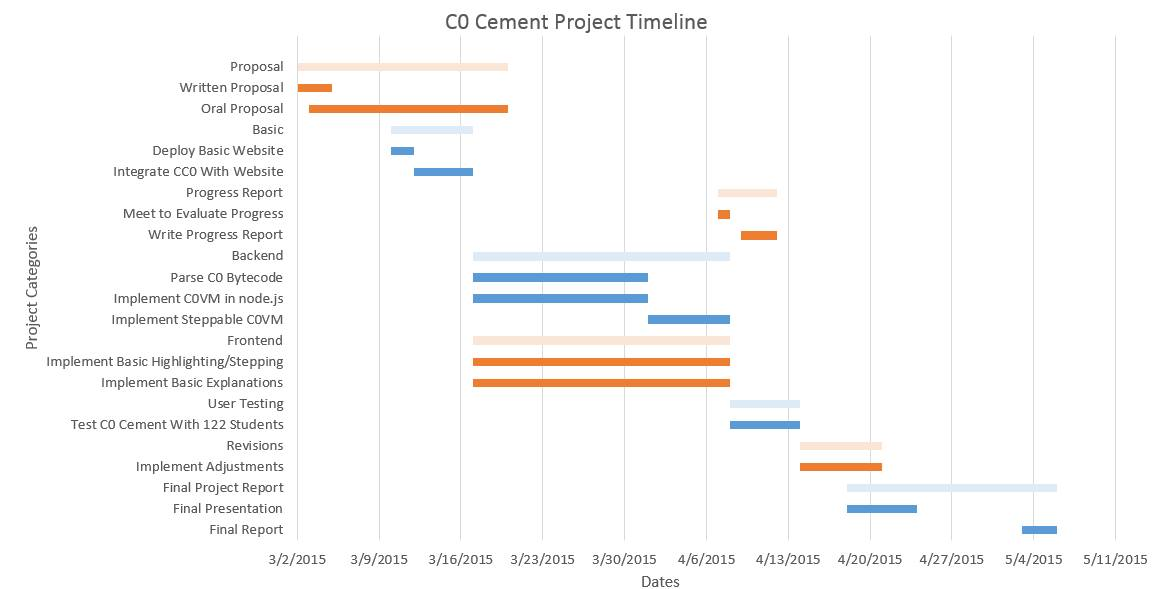
\includegraphics[width=\linewidth]{gantt.jpg}
  \caption{Project Gantt chart}
  \label{fig:gantt}
\end{figure}

\section{Evaluation Criteria}
\par
The goal of our website, as mentioned earlier in the proposal, is to provide a
tool for 15-122 students to easily step through their C0 code as a means of
debugging and to gain a deeper level of understanding for the steps their code
is actually taking.
\par
In order to evaluate our final project, we would test the product on various
groups of students.  Both those who have completed 15-122 in the past and those
currently enrolled.  Unfortunately, due to the time constraints of the project,
these students will no longer actively code in C0 by the time they see our
product, but their interactions with it will still have been recent enough for
them to provide meaningful feedback.  With their feedback, we will determine
how well our product succeeds at its aforementioned objectives and plan a
series of modifications based on the comments we receive. We will make sure
that the stepping tool and GUI are fully functional before the group testing
phase so that uninformative bugs do not catch the attention of our test
subjects, and they instead provide us with information to improve the user
experience as a whole.
\par
Our main goal is to provide these students with a useful debugging tool, so
their feedback is invaluable in modifying our project to better suit
their needs.

\section{Qualifications of Team Members}
\par
We are a team of sophomore CS majors who have varied experience in the field.
\par
Suhaas Reddy has had two years of programming experience.  He has also served
as a course assistant for the School of Computer Science for three semesters
which gives him an understanding of what computer science students may need
from a debugging tool. This spring Suhaas competed in his first Hackathon where
he and a group of three other students worked to create a webapp which
eliminated unwanted Craigslist postings from view using machine learning, and
sorted the rest based on specific attributes.  He is well-versed in Python, C0,
and C.
\par
Shyam Raghavan has had seven years of programming experience.  He has served as
a teaching assistant for the School of Computer Science for two semesters,
specifically for 15-122, which makes him especially prepared to create a
teaching tool for C0, the main language used in the course.  In the past, Shyam
has interned at Thumbtack, a west coast company which specializes in enabling
consumers to hire experience professionals from a variety of fields.  Shyam has
experience with C, JavaScript, and C0.
\par
Aaron Gutierrez has had ten years of programming experience.  He has also served
as a teaching assistant for the School of Computer Science for two semesters in
15-122 with Shyam. This past summer Aaron worked at Orion Pipeline developing
web applications for real-time resource monitoring. Aaron is very well-versed in
JavaScript, C, and C0.
\par
Mitchell Plamann has had nine years of programming experience.  For the past two
summers, he interned at Rockwell Automation, doing firmware developement for
embedded systems. Mitchell has coded extensively in C, C0, and Haskell.
% You know I had to say it, right?

\section{Sources Cited}
\begin{enumerate}
\item Amjad Masad,
  ``Building an In-Browser JavaScript VM and Debugger Using Generators'',\\
  http://amasad.me/2014/01/06/building-an-in-browser-javascript-vm-and-debugger-using-generators/
\item Mike Kamermans, ``The Architecture of Open Source Applications (Volume 2)'',\\
  http://www.aosabook.org/en/pjs.html
\item Joyent, Inc., ``Node.js Documentation'', \\
  http://nodejs.org/documentation
\end{enumerate}

\end{document}
